%%%%%%%%%%%%%%%%%%%%%%%%%%%%%%%%%%%%%%%%%%%%%%%%%%%%%%%%%%
%
% Authors: Gautam Ramesh, Siddanth Sharma, Shubhankar Dumka
% File: HardwareAssembly.tex
% Version: 9.0 (optimized Structure)
% Description: Detailed assembly with upfront Port Mapping
%
%%%%%%%%%%%%%%%%%%%%%%%%%%%%%%%%%%%%%%%%%%%%%%%%%%%%%%%%%%

\chapter{Hardware Assembly and System Commissioning}

This chapter serves as the definitive engineering guide for the physical construction, integration, and environmental calibration of the License Plate Detection System. Unlike standard consumer electronics, this edge-AI device requires strict adherence to assembly protocols to ensure thermal stability, data integrity, and optical precision.

\section{Site Preparation and Safety Protocols}
Before unpacking the components, the installation site must be validated against the engineering constraints defined in the project safety matrix.

\subsection{Environmental Prerequisites}
\begin{itemize}
	\item \textbf{Illumination:} The detection zone must maintain a lighting level between \textbf{250 lux (minimum)} and \textbf{900 lux (maximum)}. For optimal Optical Character Recognition (OCR) accuracy, a target range of \textbf{400--700 lux} is recommended.
	\item \textbf{Thermal Envelope:} The ambient temperature must remain between \SI{0}{\celsius} and \SI{40}{\celsius}. If deploying in direct sunlight, a shaded enclosure is mandatory to prevent thermal throttling of the NVIDIA Maxwell GPU.
	\item \textbf{Power Stability:} A dedicated wall outlet capable of supplying continuous \SI{5}{\volt}/\SI{4}{\ampere} without voltage sag is strictly required.
\end{itemize}

\subsection{ESD and Handling Precautions}
The reComputer J1010 contains sensitive CMOS components.
\begin{table}[H]
	\centering
	\caption{Mandatory Safety Precautions}
	\begin{tabular}{|p{4cm}|p{10cm}|}
		\hline
		\textbf{Hazard} & \textbf{Preventative Measure} \\ \hline
		Electrostatic Discharge & Wear an ESD wrist strap or touch a grounded metal object before handling the Main Unit. \\ \hline
		Physical Shock & Do not drop the camera module; the lens focus mechanism is fragile. \\ \hline
		Thermal Burns & Do not touch the internal heatsink immediately after operation. \\ \hline
	\end{tabular}
\end{table}

\newpage
% =================================================================
% MASTER INVENTORY
% =================================================================
\section{Master Component Inventory}
Refer to the visual inventory in Figure \ref{fig:master_parts}. Ensure all 9 subsystems are present before proceeding.

\begin{figure}[H]
	\centering
	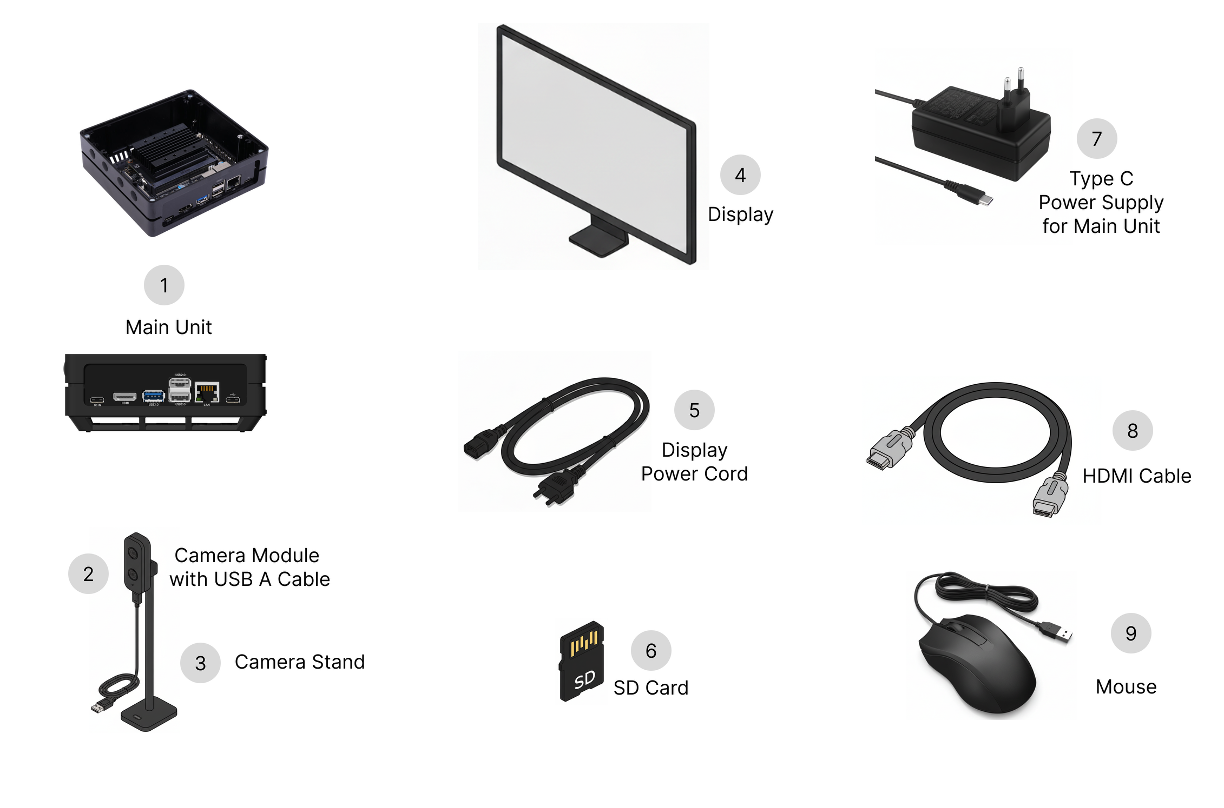
\includegraphics[width=1.0\textwidth]{images/ListOfParts.png}
	\caption{Master System Inventory: Components 1 through 9.}
	\label{fig:master_parts}
\end{figure}

\begin{table}[H]
	\centering
	\caption{Bill of Materials (BOM) Definitions}
	\begin{tabular}{|l|l|l|}
		\hline
		\textbf{ID} & \textbf{Component} & \textbf{Function} \\ \hline
		1 & Main Unit & Central AI Processing Core (Seeed reComputer) \\ \hline
		2 & Camera Module & Image Acquisition (Microsoft LifeCam) \\ \hline
		3 & Camera Stand & Optical Geometry Stabilization \\ \hline
		4 & Display & User Interface Visualization \\ \hline
		5 & Power Cord & Display Power \\ \hline
		6 & SD Card & Operating System \& Storage Media \\ \hline
		7 & Power Supply & System Power (5V/4A Type-C) \\ \hline
		8 & HDMI Cable & Video Signal Transmission \\ \hline
		9 & Mouse & Human Interface Device (HID) \\ \hline
	\end{tabular}
\end{table}

\newpage
% =================================================================
% PORT REFERENCE (MOVED TO FRONT)
% =================================================================
\section{Main Unit Interface Map}
The reComputer J1010 features distinct communication buses. Identifying the correct ports \textbf{before assembly} is critical for system performance.

\begin{figure}[H]
	\centering
	
\includegraphics[width=0.85\textwidth]{images/jetsonNanoPorts.png}
	\caption{Rear I/O Layout. Note the distinction between the Blue (High-Speed) and Black (Standard) USB ports.}
	\label{fig:rear_ports}
\end{figure}

\begin{itemize}
	\item \textbf{DC IN (USB-C):} Dedicated power input. Do NOT use for data.
	\item \textbf{HDMI:} Primary video output for the dashboard monitor.
	\item \textbf{USB 3.0 (Blue):} High-bandwidth bus (5Gbps). \textit{Reserved for Camera and SSD.}
	\item \textbf{USB 2.0 (Black):} Low-bandwidth bus. \textit{Reserved for Mouse and Keyboard.}
\end{itemize}

\newpage
% =================================================================
% MAIN UNIT INSTALLATION
% =================================================================
\section{Compute Core Installation (Main Unit)}

\subsection{Component Profile}
The \textbf{Seeed Studio reComputer J1010} acts as the central processing brain. It houses the NVIDIA Jetson Nano module and the J101 carrier board within an aluminum enclosure.

\subsection{Internal Inspection}
Before connecting any cables, inspect the internal layout to ensure the heatsink is seated correctly.

\begin{figure}[H]
	\centering
	
\includegraphics[width=0.8\textwidth]{images/jetsonHardware.jpg}
	\caption{Internal anatomy of the J101 carrier board showing the passive heatsink assembly.}
\end{figure}

\subsection{Placement Strategy}
Place the Main Unit on a flat, non-conductive surface. Ensure a minimum clearance of \textbf{10 cm} on all sides to allow for passive airflow through the chassis vents.

\begin{figure}[H]
	\centering
	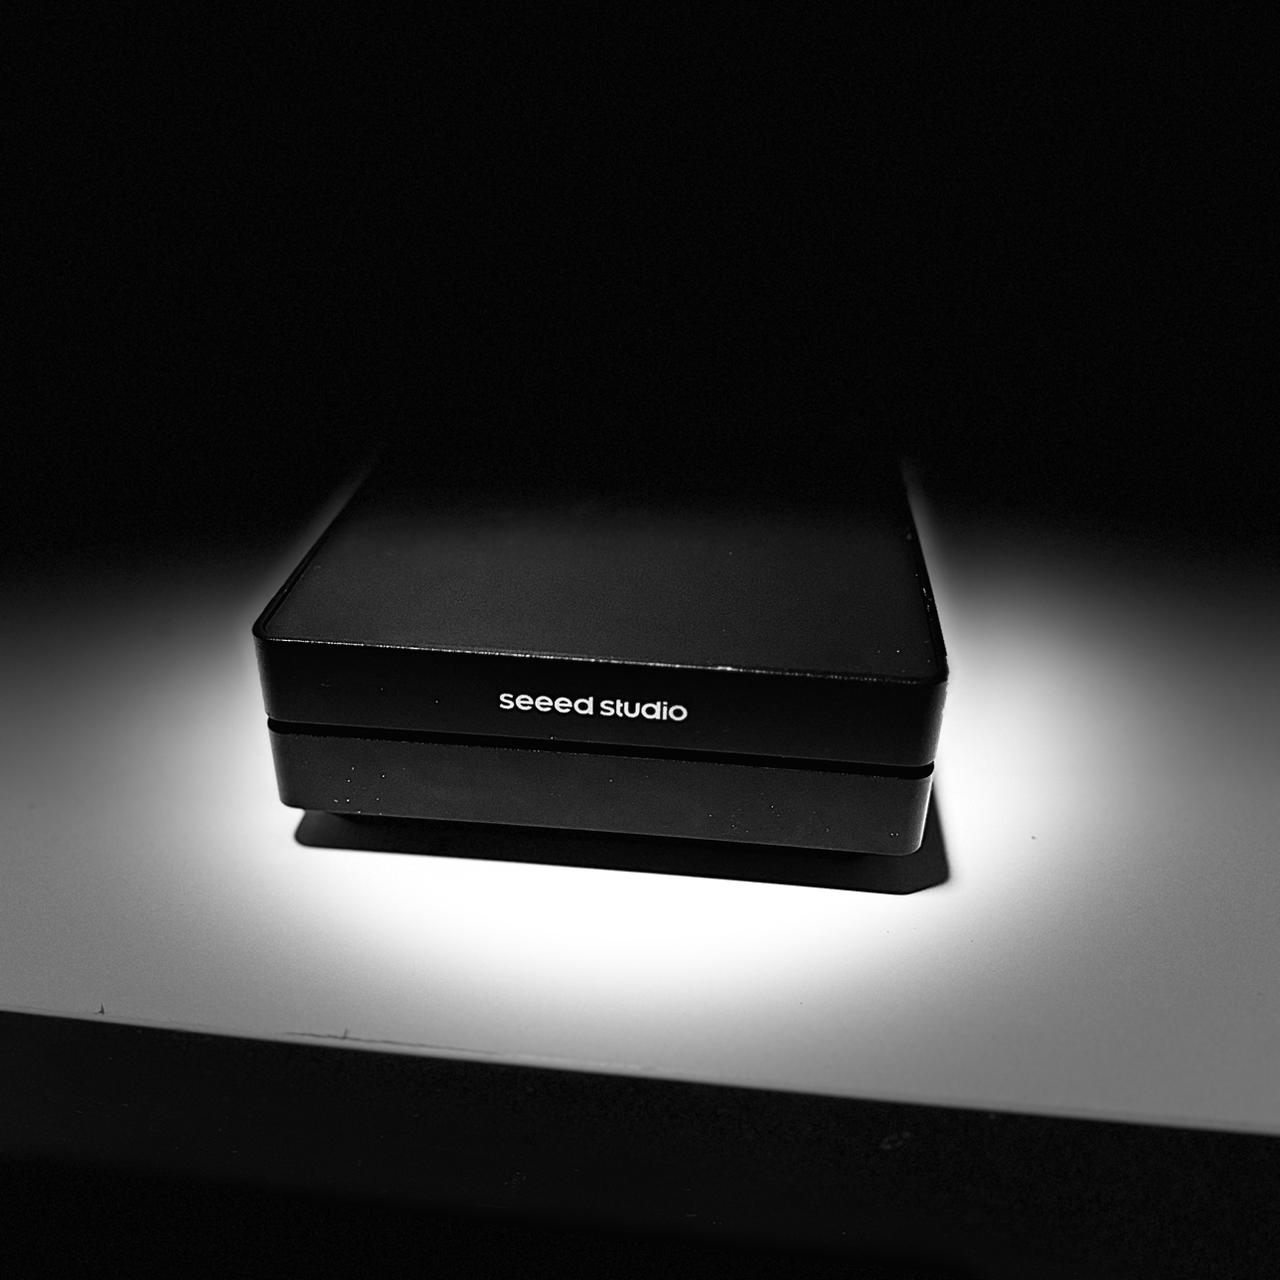
\includegraphics[width=0.6\textwidth]{images/JetsonNano.jpeg}
	\caption{Correct orientation of the Main Unit on the workbench.}
\end{figure}

% =================================================================
% SD CARD
% =================================================================
\section{Operating System Media (SD Card)}

\subsection{Component Profile}
The system utilizes a \SI{32}{GB} (or larger) Class 10 UHS-I Micro-SD card containing the Ubuntu OS, JetPack 5.1.2 drivers, and the custom YOLOv8 inference engine.

\subsection{Installation Procedure}
\textbf{Critical Warning:} This step must be performed \textit{before} connecting power. Hot-plugging the SD card can corrupt the file system.

\begin{enumerate}
	\item Locate the spring-loaded slot on the underside of the Main Unit carrier board.
	\item Orient the card so the text faces \textbf{down} and the gold pins face \textbf{up} (toward the internal heatsink).
	\item Gently slide the card into the slot.
	\item Press firmly until a physical "click" is felt, indicating the card is locked into the retention mechanism.
\end{enumerate}

\begin{figure}[H]
	\centering
	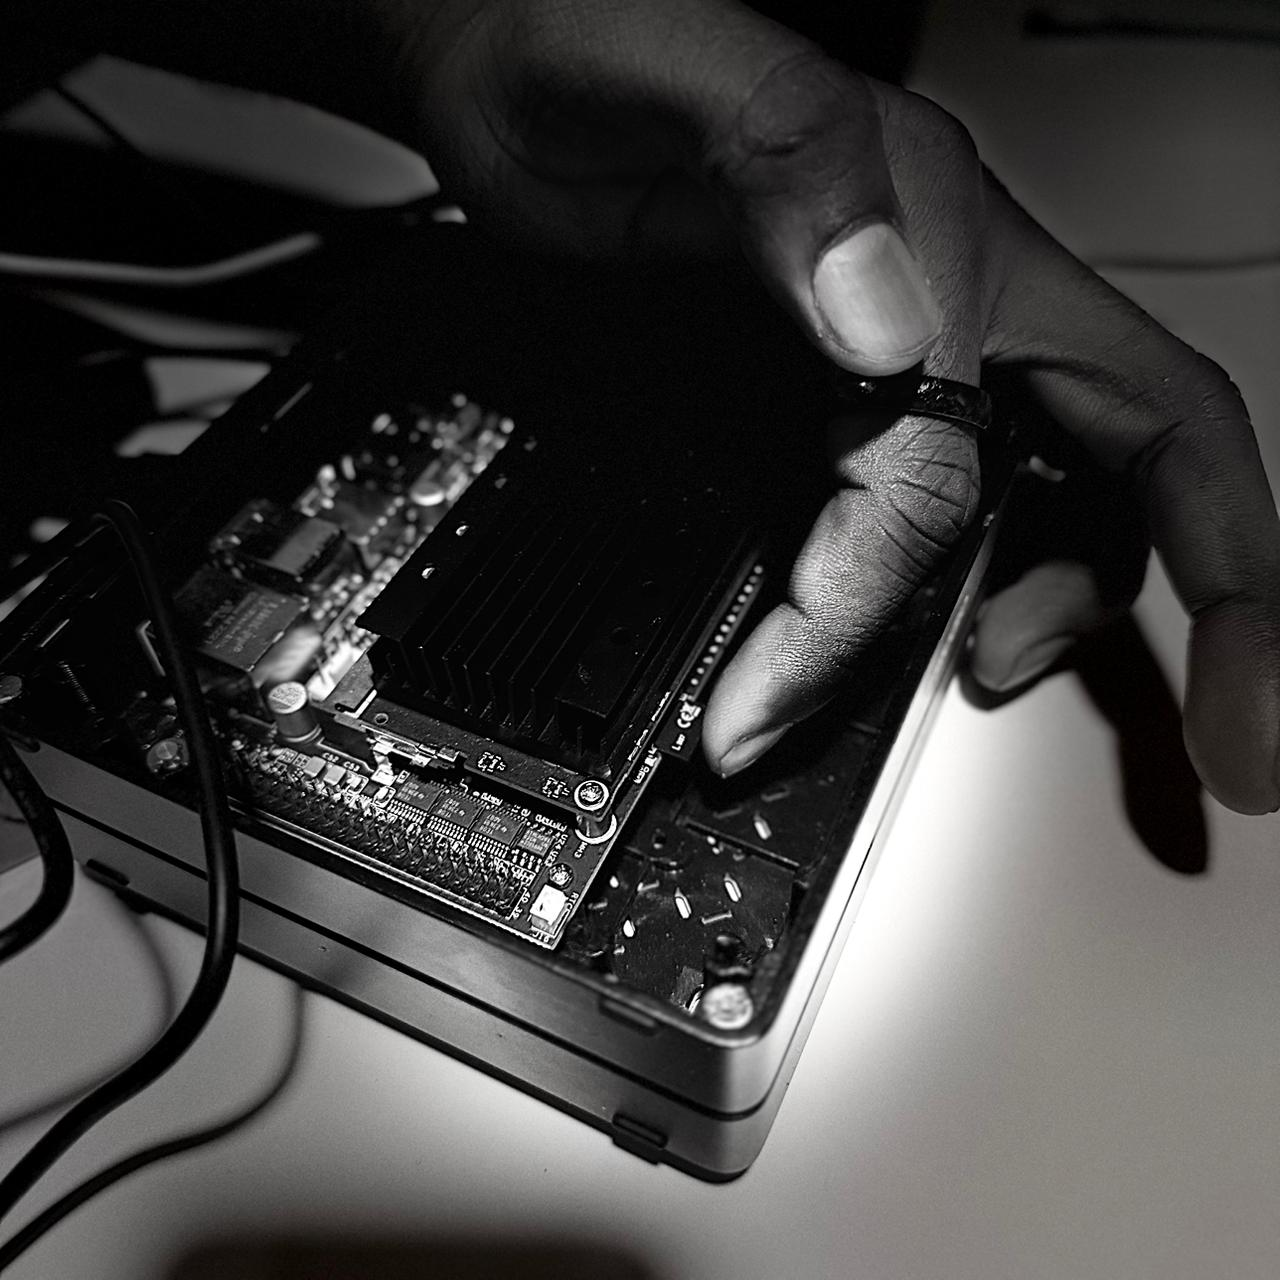
\includegraphics[width=0.7\textwidth]{images/SdCard.jpeg}
	\caption{Manual insertion of the SD Card. Note the user handling the board edges to avoid ESD.}
\end{figure}

\newpage
% =================================================================
% OPTICAL SUBSYSTEM
% =================================================================
\section{Optical Subsystem Setup (Camera)}

\subsection{Component Profile}
The Microsoft LifeCam (1080p@30fps) is mounted on an adjustable stand to provide the raw video feed for the AI.

\subsection{Physical Mounting}
Attach the camera clip to the head of the stand. Ensure the camera is level and the lens is free of fingerprints.

\begin{figure}[H]
	\centering
	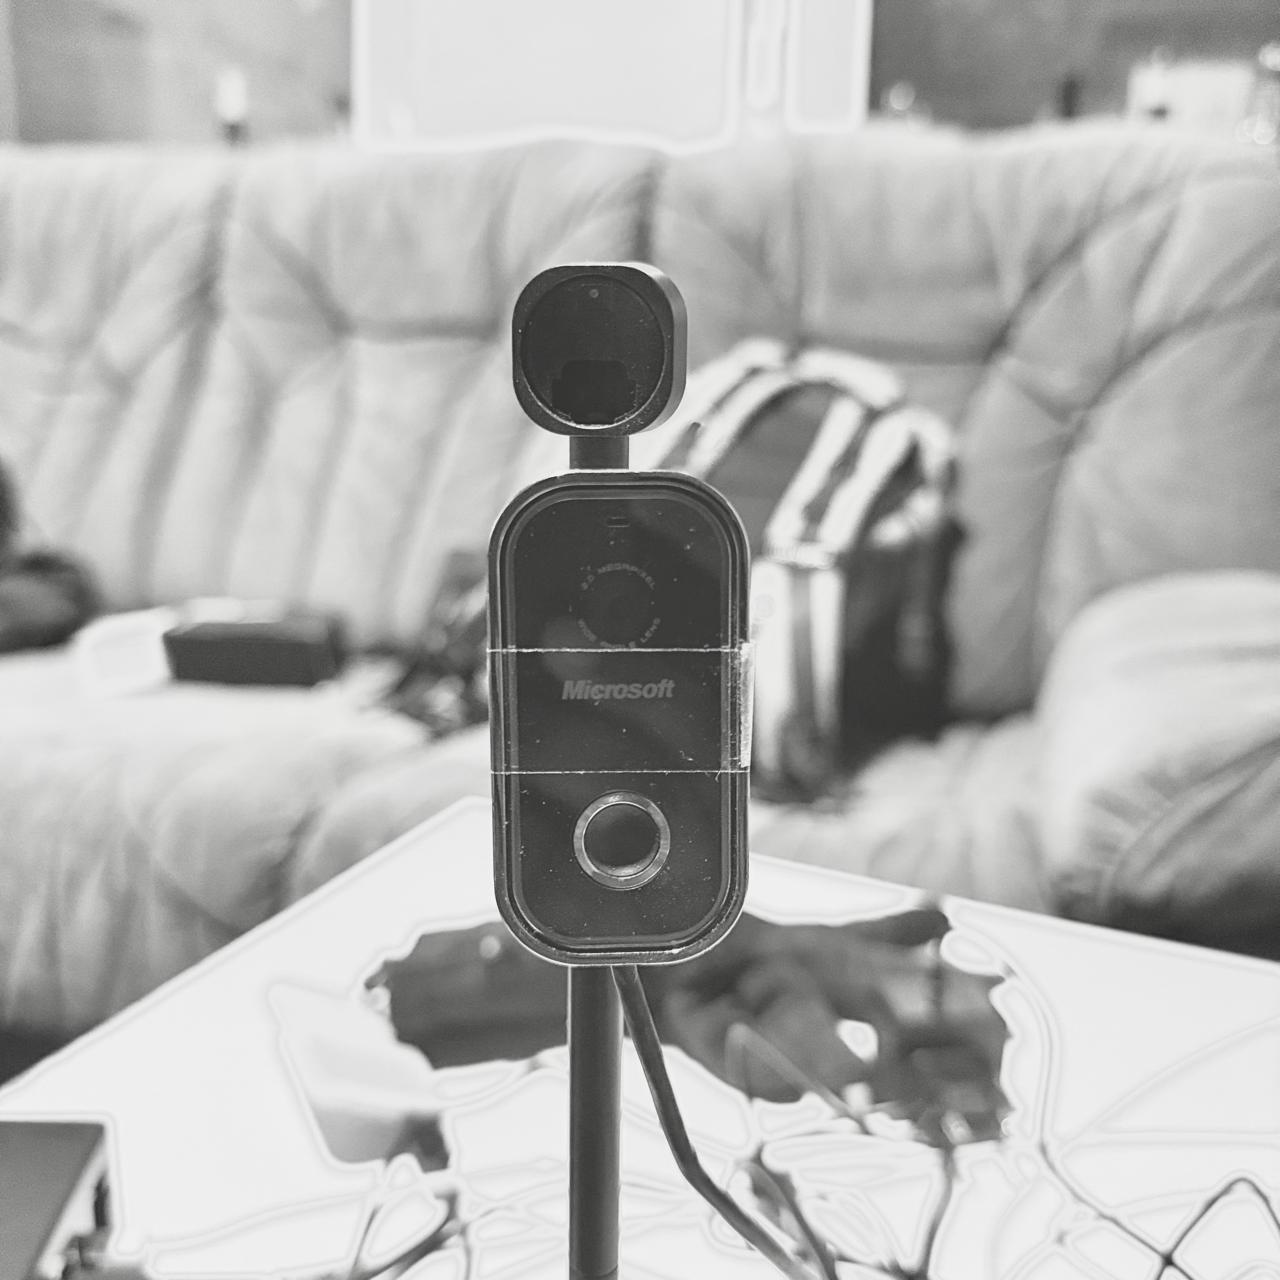
\includegraphics[width=0.55\textwidth]{images/camera.jpeg}
	\caption{Camera module mounted on the stand, ready for calibration.}
\end{figure}

\subsection{Optical Calibration Metrics}
To ensure the OCR software can read German license plates, the camera must be positioned according to strict geometric constraints:

\begin{table}[H]
	\centering
	\caption{Optical Calibration Standards (Ref: Section 2.2 Operational Setup)}
	\begin{tabular}{|l|l|l|}
		\hline
		\textbf{Metric} & \textbf{Value Range} & \textbf{Tolerance} \\ \hline
		\textbf{Mounting Height} & 2.0 meters -- 2.5 meters & $\pm$ 10 cm \\ \hline
		\textbf{Detection Distance} & 3.0 meters -- 5.0 meters & $\pm$ 50 cm \\ \hline
		\textbf{Vertical Inclination} & 30\textdegree -- 40\textdegree & $\pm$ 5\textdegree \\ \hline
	\end{tabular}
\end{table}

\newpage
\subsection{Data Connection (USB 3.0)}
The camera requires high-bandwidth communication. Refer to the Interface Map (Figure \ref{fig:rear_ports}) for port location.

\begin{enumerate}
	\item Identify the **Blue USB 3.0** port on the rear panel.
	\item Insert the camera's USB Type-A connector into this port.
	\item \textbf{Verification:} Ensure the connector is fully seated. Loose cables will cause video signal dropouts.
\end{enumerate}

\begin{figure}[H]
	\centering
	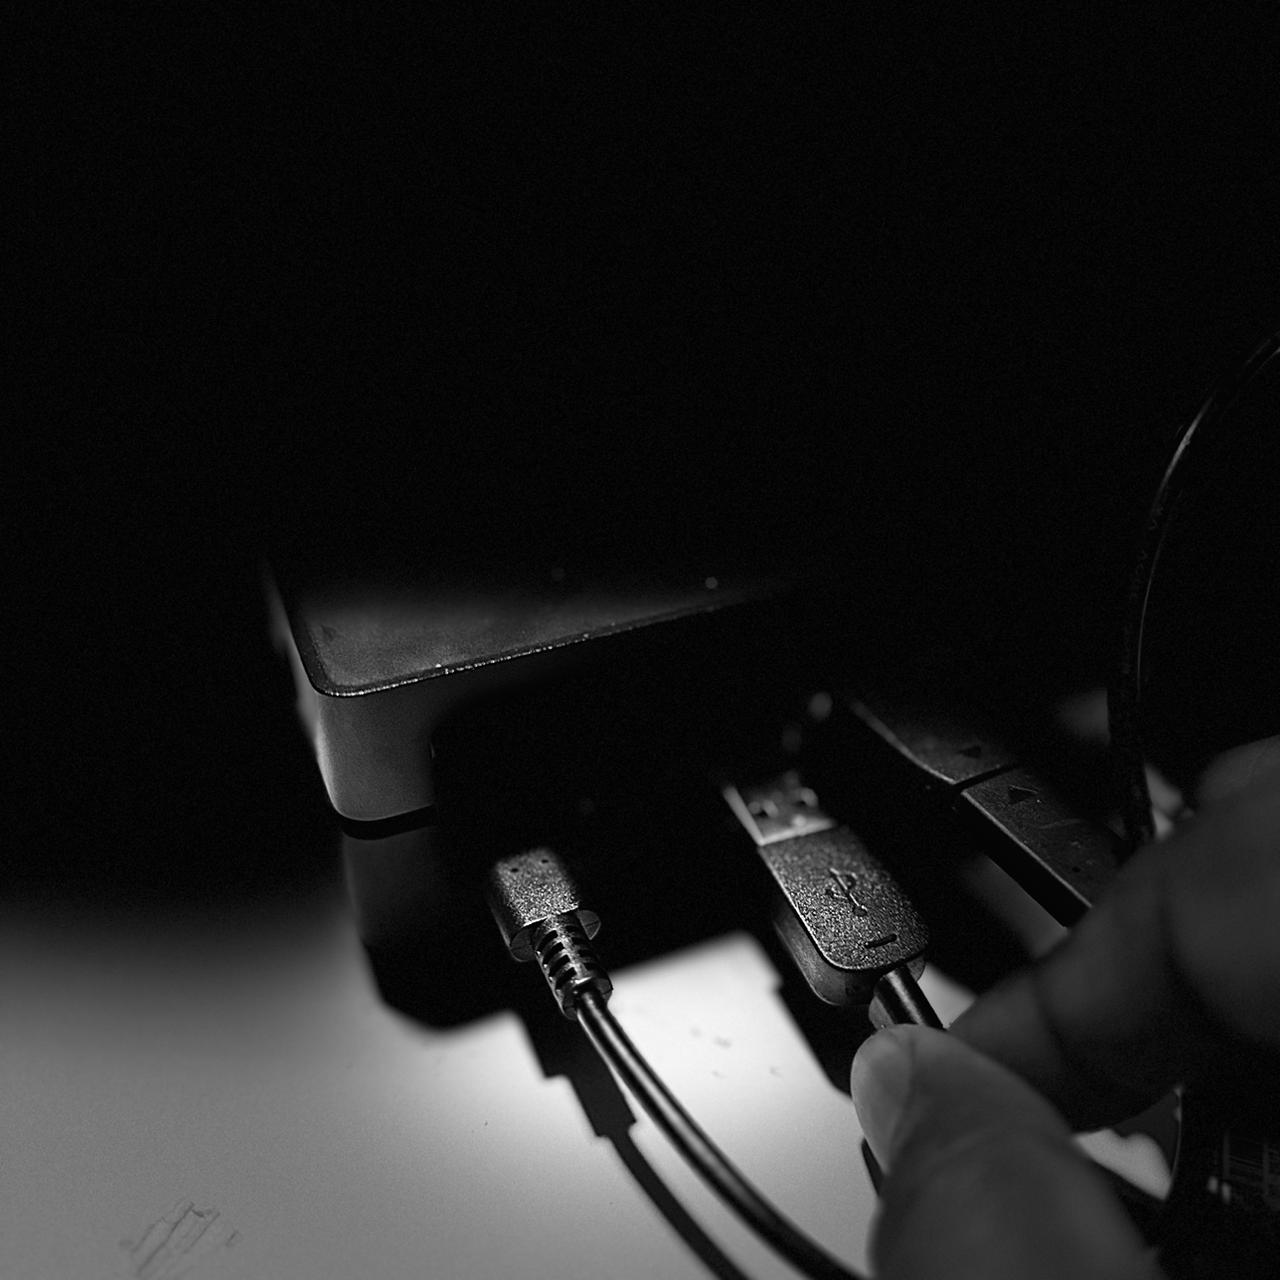
\includegraphics[width=0.7\textwidth]{images/usbConnection.jpeg}
	\caption{Connecting the Camera data cable to the Blue USB 3.0 High-Speed port.}
\end{figure}

\newpage
% =================================================================
% VISUALIZATION
% =================================================================
\section{Visualization Subsystem (Display)}

\subsection{Display Integration}
The operator dashboard is viewed via an external HDMI Monitor.
\begin{figure}[H]
	\centering
	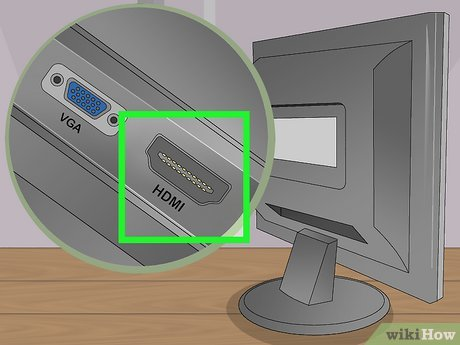
\includegraphics[width=0.7\textwidth]{images/hdmiMoniter.jpg}
	\caption{Connecting the Camera data cable to the Blue USB 3.0 High-Speed port.}
\end{figure}
\begin{enumerate}
	\item Connect the HDMI Cable to the \textbf{HDMI Port} (Ref: Figure \ref{fig:rear_ports}) on the rear of the Main Unit.
	\item Connect the other end to the Monitor.
	\item Connect the Power Cord to the Monitor and the wall outlet.
\end{enumerate}

\begin{quote}
	\textbf{Note:} Power on the monitor \textit{before} the Main Unit to ensure the resolution (1920x1080) is auto-detected correctly.
\end{quote}

% =================================================================
% USER INPUT
% =================================================================
\section{Human Interface Devices (Mouse/Keyboard)}

\subsection{Installation}
A standard USB mouse and keyboard are required for interacting with the GUI, specifically for the system login and "Shutdown" operation.

\begin{itemize}
	\item Connect the Mouse and Keyboard to any available \textbf{Black USB 2.0} port.
	\item \textbf{Note:} Do not use the Blue ports for these devices; save those bandwidth-heavy ports for the Camera and SSD.
\end{itemize}

\begin{figure}[H]
	\centering
	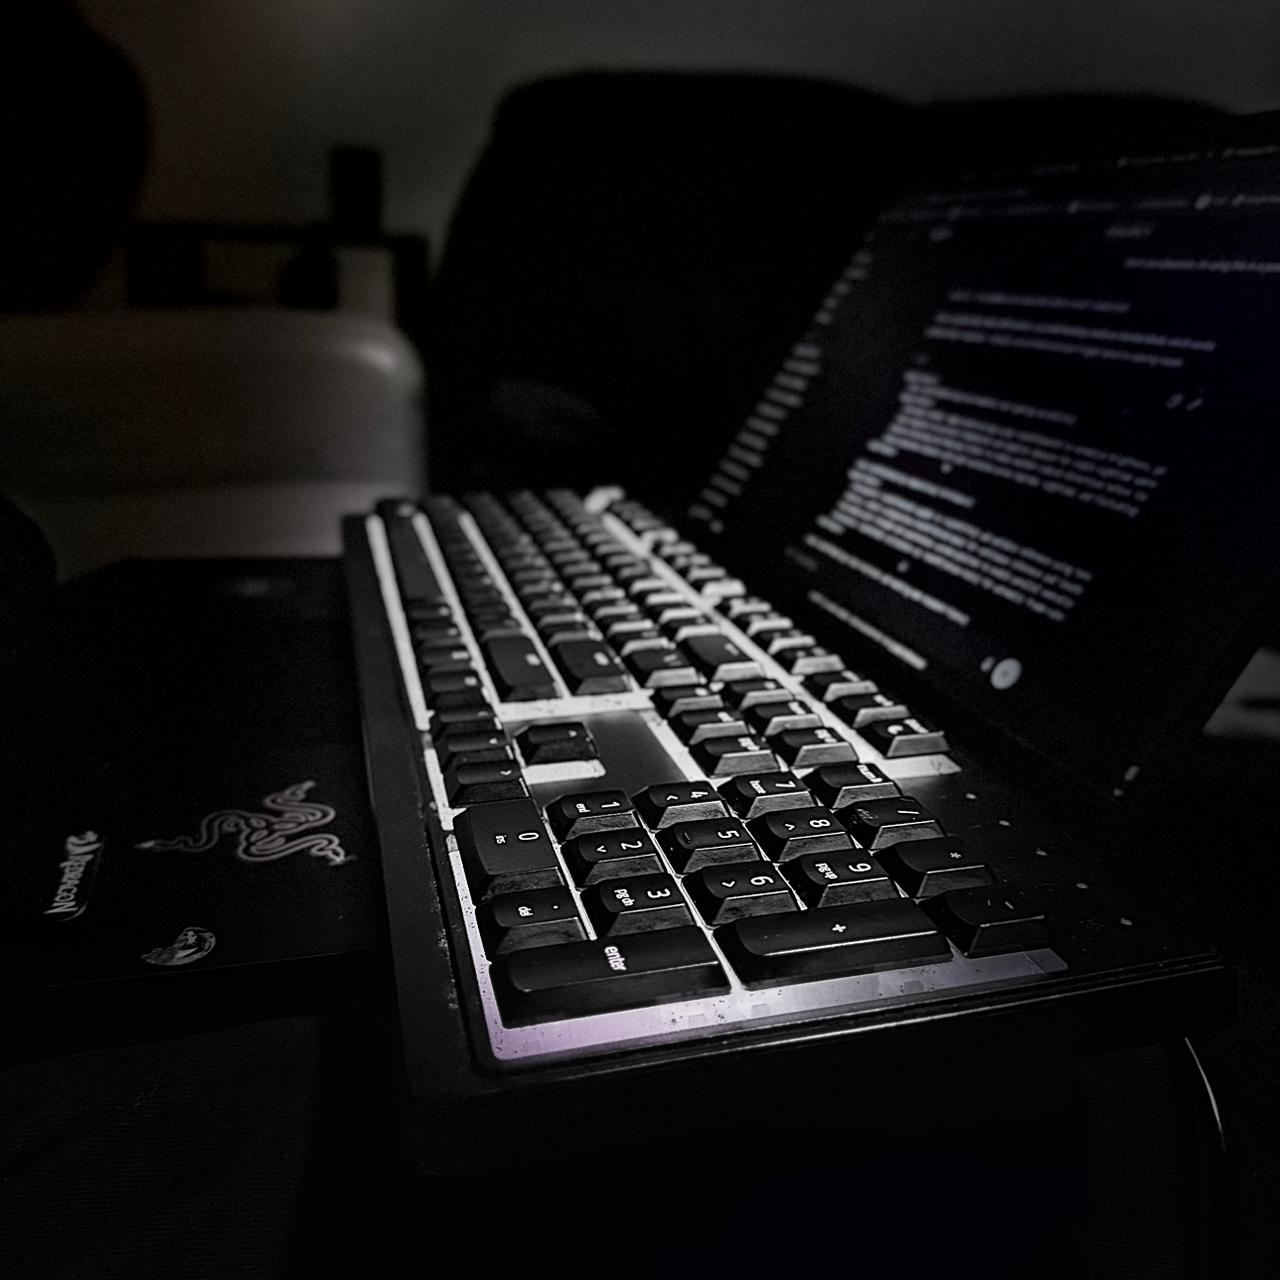
\includegraphics[width=0.7\textwidth]{images/Keyboard.jpeg}
	\caption{Connecting User Input devices to the secondary USB bus.}
\end{figure}

\newpage
% =================================================================
% POWER SUPPLY
% =================================================================
\section{Power Regulation Subsystem}

\subsection{Component Profile}
The system uses a \SI{5}{\volt}/\SI{4}{\ampere} Type-C Power Adapter. It is the critical life-support system for the AI inference engine.

\subsection{Connection Protocol (Device Side)}
\textbf{Warning:} Do not force the connector. Ensure alignment with the port labeled \textbf{"DC IN"}. Do not use the other USB-C port labeled "OTG" or "USB" for power.

\begin{figure}[H]
	\centering
	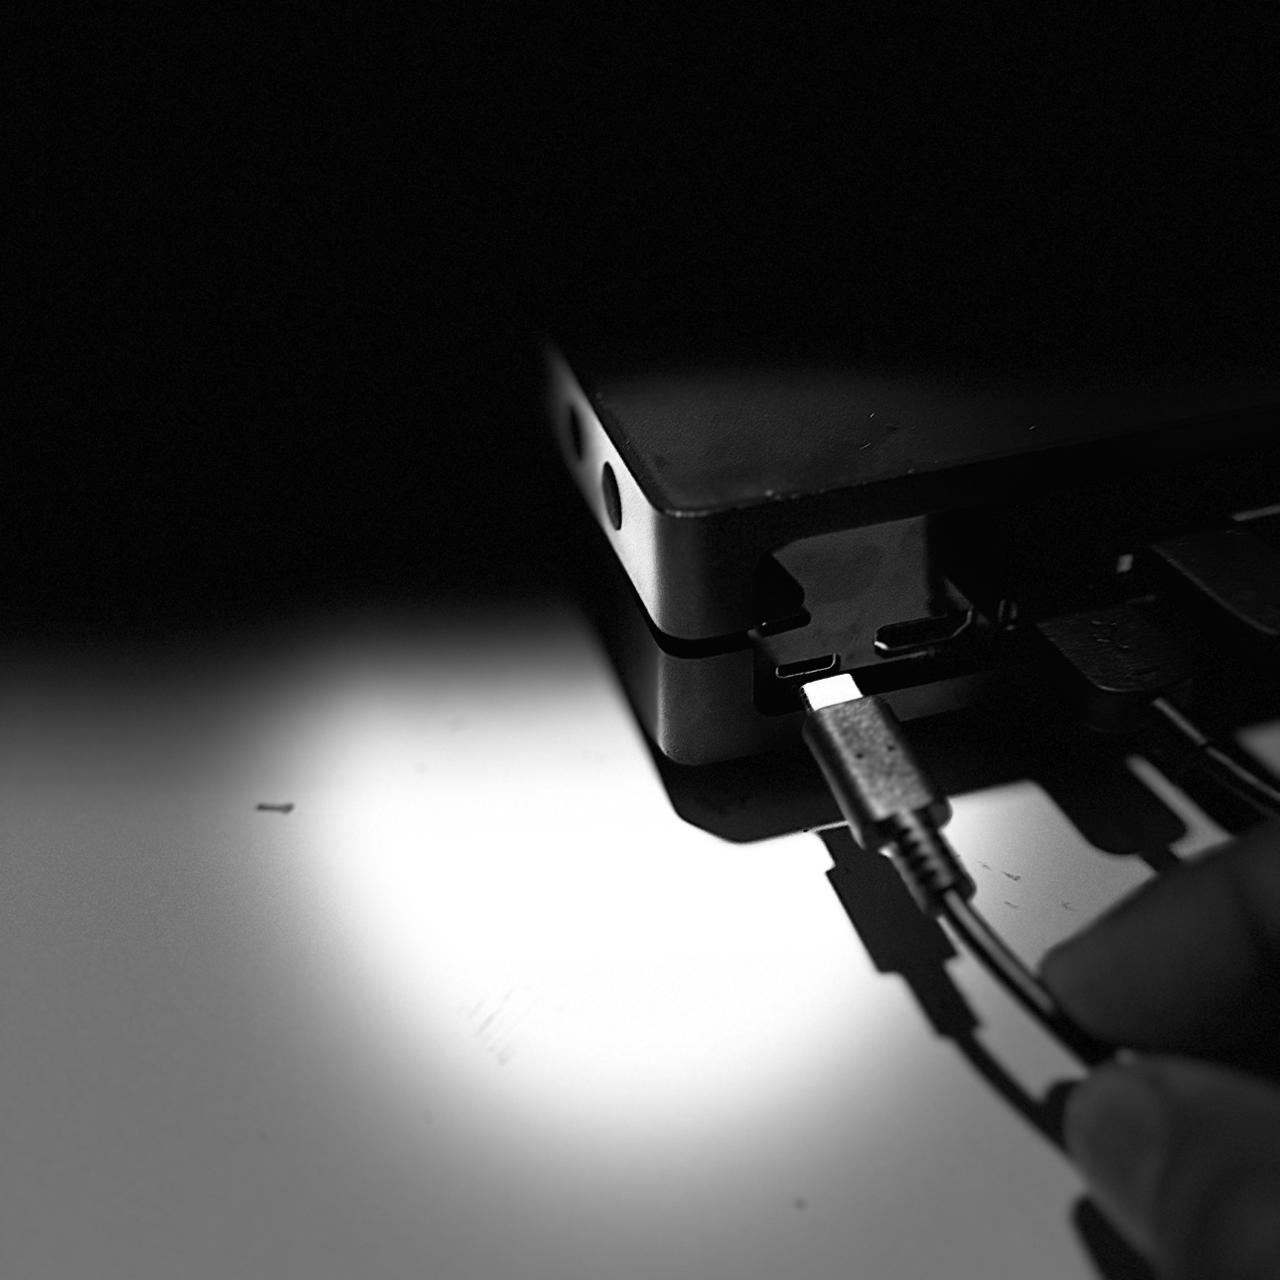
\includegraphics[width=0.65\textwidth]{images/powerTypecConnection.jpeg}
	\caption{Inserting the Type-C connector into the dedicated DC-IN port.}
\end{figure}

\subsection{Connection Protocol (Wall Side)}
\begin{figure}[H]
	\centering
	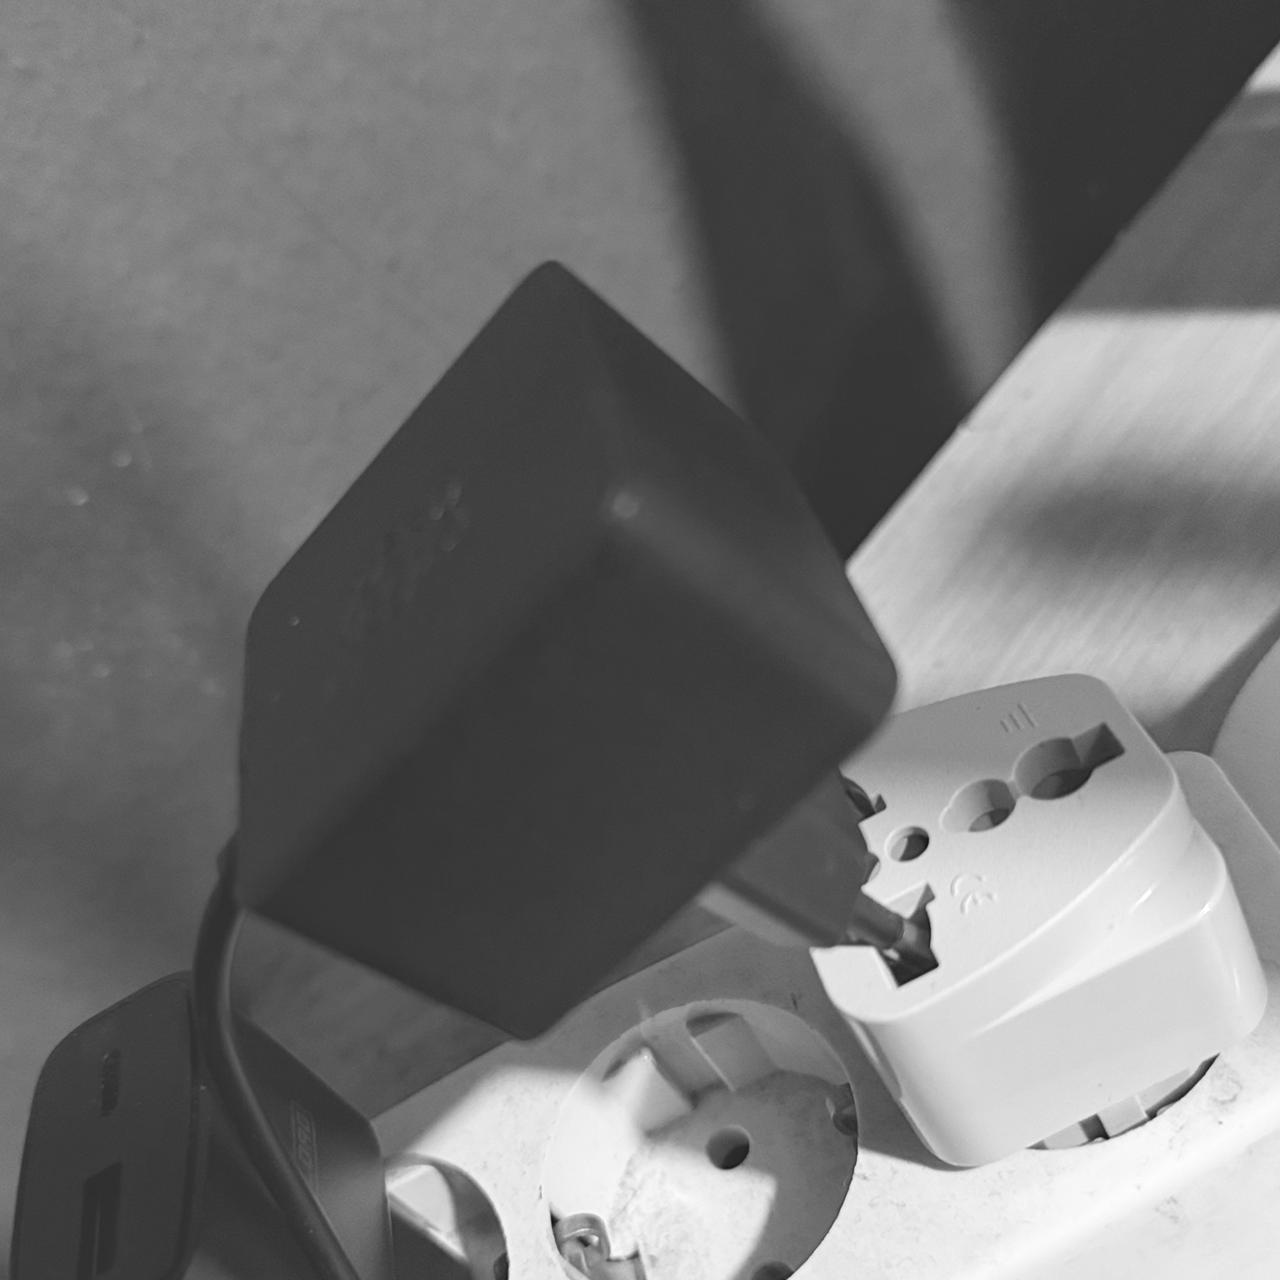
\includegraphics[width=0.6\textwidth]{images/Adapter.jpeg}
	\caption{Final connection to the AC mains source.}
\end{figure}
\begin{enumerate}
	\item Connect the adapter block to the mains wall socket.
	\item \textbf{Verification:} A Green LED on the Main Unit chassis will illuminate immediately.
\end{enumerate}



\newpage
% =================================================================
% SOFTWARE STARTUP
% =================================================================
\section{First Boot and Initialization}
\begin{figure}[H]
	\centering
	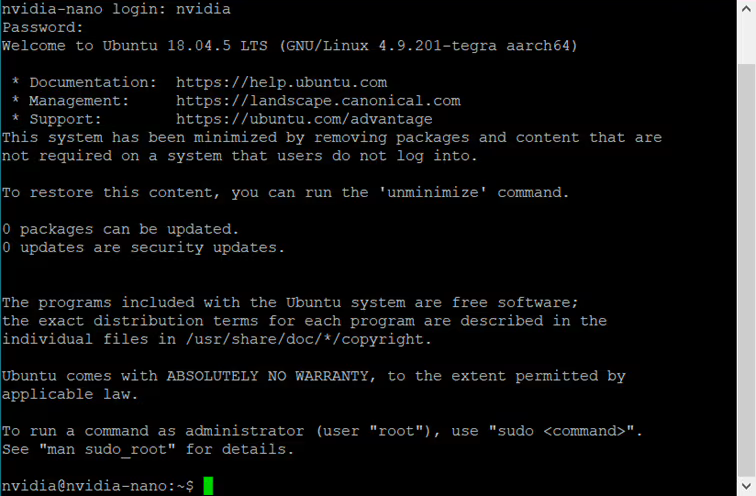
\includegraphics[width=0.7\textwidth]{images/terminal.png}
	\caption{Login Terminal}
\end{figure}
Once all hardware components are integrated and powered, the system requires an initial software login to launch the Operator Dashboard.

\subsection{System Login}
The device will boot into a text-based terminal environment.
\begin{enumerate}
	\item When prompted for \texttt{recomputer login:}, type \textbf{\texttt{nvidia}} and press Enter.
	\item When prompted for \texttt{Password:}, type \textbf{\texttt{nvidia}} and press Enter.
	\item \textit{Note: Password characters will not appear on screen for security.}
\end{enumerate}

\subsection{Launching the Interface}
To start the graphical environment and the License Plate Detection software:
\begin{enumerate}
	\item At the command prompt (\texttt{\$}), type:
	\begin{verbatim}
		startx
	\end{verbatim}
	\item Press \textbf{Enter}.
	\item The screen will flicker briefly before loading the full desktop environment and automatically opening the monitoring dashboard.
\end{enumerate}

\noindent
\textbf{Commissioning Complete:} The system is now fully assembled, powered, and operational. Proceed to the "Operation Manual" chapter for usage instructions.